\hypertarget{introduction}{%
\section{Introduction}\label{introduction}}

Modern computers provide many proactive security measures to defend
against attacks. These protections can either be implemented at the
hardware level (such as data execution prevention) or the
software/operating system level (such as address space layout
randomisation and sandboxing).

\hypertarget{data-execution-prevention}{%
\subsection{Data Execution Prevention}\label{data-execution-prevention}}

Data Execution Prevention (DEP) is a hardware feature supported by
modern CPUs which mark certain memory locations, such as the process
stack and heap, as non-executable (i.e.~code in these sections of memory
cannot be executed). The exact mechanism varies depending on the CPU
architecture, but it is implemented in x86\_64 CPUs with the NX
(no-execute, defined by AMD)/XD (execute disable, defined by Intel) bit.
By marking these memory segments as non-executable, the CPU can defend
against attacks which rely on inserting shellcode into a buffer such as
buffer overflow attacks and code injection attacks.

This can be demonstrated using an extremely basic C program and the
assistance of GDB (though any C debugger should work for this). The
program only needs to contain an allocated buffer, which can be done by
initialising an empty array of any arbitrary size.

\begin{verbatim}
int main() {
    int integers[64];
}
\end{verbatim}

This needs to be compiled with debugging symbols enabled (with the
\texttt{-g} compilation flag) to make debugging the program easier. By
default, the binary produced will have a non-executable stack (i.e.~the
stack's memory cannot be executed). The produced binary can then be
analysed using \texttt{gdb}.

In the GDB interface, a breakpoint must be established after the buffer
declaration but before the program terminates. This can be done using
\texttt{b\ 2}, which sets a breakpoint at the third line of the program.
Once the breakpoint has been established, the program can be run using
\texttt{r} which will automatically pause execution at the breakpoint.

\begin{figure}
\centering
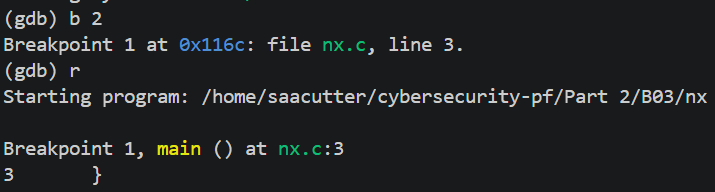
\includegraphics{nx/nx_br.png}
\caption{nx\_break\_run}
\end{figure}

At this point, the buffer has been initialised so it has a memory
address. This memory address can be accessed using
\texttt{p\ \&integers}.

\begin{figure}
\centering
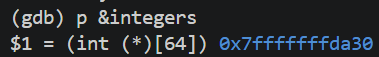
\includegraphics{nx/nx_p.png}
\caption{nx\_print\_integers}
\end{figure}

Now that the memory address of the buffer is known, it can have some
shellcode instructions assigned to it. Any instruction could be used,
but for this demonstration the \texttt{NOP} instruction (which has the
opcode \texttt{0x90}) will be used because it only increments the
\texttt{rip} instruction pointer to the next memory address. The
\texttt{rip} register stores the address of the next instruction to be
executed, so setting it to the start of this buffer will cause it to
start executing the instructions inside the buffer sequentially.

\begin{figure}
\centering
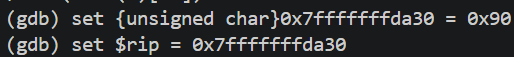
\includegraphics{nx/nx_rip.png}
\caption{nx\_rip\_set}
\end{figure}

Now that the preparation is complete, the program can continue running
with \texttt{c}.

\begin{figure}
\centering
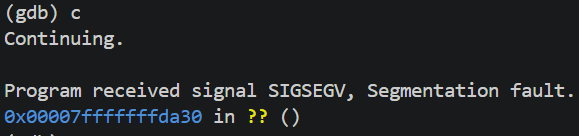
\includegraphics{nx/nx_nonexec_segfault.png}
\caption{nx\_nonexecutable\_segfault}
\end{figure}

This results in a segmentation fault being raised at the address of the
buffer because it is not executable, as expected. This binary can now be
recompiled, ensuring that the stack is made executable using the
\texttt{-z\ execstack} compilation option, and this process repeated.

\begin{figure}
\centering
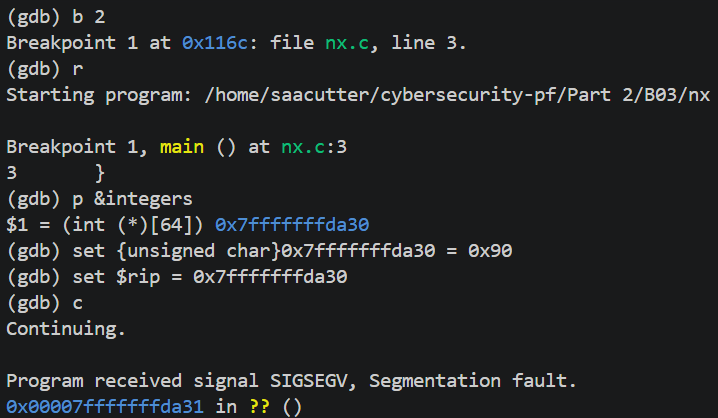
\includegraphics{nx/nx_exec_segfault.png}
\caption{nx\_executable\_segfault}
\end{figure}

Notably, the segmentation fault occurred at one memory address beyond
the initial buffer address. This is actually behaving as expected
because the \texttt{NOP} instructions continuously advance the
instruction pointer through memory until it eventually reaches an
invalid or inaccessible section of memory, resulting in a segmentation
fault. Since arrays in C occupy contiguous regions of memory, the
instruction pointer advances sequentially through the buffer until it
eventually reaches unmapped memory. To confirm this, a smaller buffer
can be used with every element of the buffer filled with \texttt{NOP}
instructions.

\begin{figure}
\centering
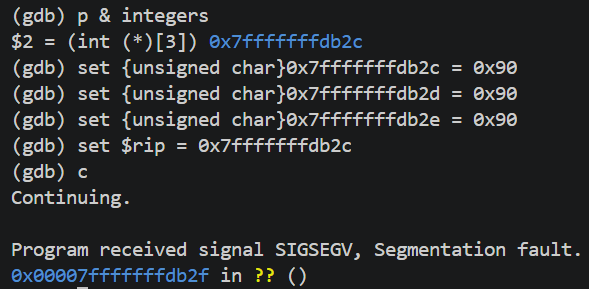
\includegraphics{nx/nx_exec_bufferfill.png}
\caption{nx\_exec\_buffer\_overflow}
\end{figure}

In this case, the segmentation fault signal was raised at
\texttt{0x7fffffffdb2f} which is 4 positions after the initial memory
address (\texttt{0x7fffffffdb2c\ +\ 4\ =\ 0x7fffffffdb2f}). This occurs
because the \texttt{NOP} instruction increments the instruction pointer
sequentially through the array until it eventually reaches unmapped
memory, resulting in a segmentation fault.

It is evident that making the stack executable should only be done in
circumstances where the consequences are known, as \texttt{gcc} (and
other C compilers) will proactively make the stack non-executable. If
these executable memory protections are disabled, attackers could inject
and execute malicious shellcode within writable memory regions (like
buffers). This is the basic idea behind buffer overflow and code
injection attacks.

\hypertarget{address-space-layout-randomisation}{%
\subsection{Address Space Layout
Randomisation}\label{address-space-layout-randomisation}}

Address Space Layout Randomisation (ASLR) is a security mechanism
implemented in modern operating systems which randomises the memory
locations used by processes, libraries, stacks, heaps, and other
allocated memory regions. This makes it harder for attackers to predict
where code will load, which makes exploits harder to perform. This helps
defend against many memory-based exploits, such as buffer overflow and
code injection attacks, which rely on knowing the exact addresses of
data in the system's memory to execute the attack (often in the form of
``shellcode'').

This can be tested using a basic C program which allocates heap memory
and prints the memory address of the pointer.

\begin{verbatim}
#include <stdio.h>
#include <stdlib.h>

int main(void) {
    int *p = (int *)malloc(sizeof(int));
    printf("%p\n", p);
    free(p); // not necessary but stops memory leaks
}
\end{verbatim}

After compiling this program, the memory address that gets printed will
change every time the program is run. This change makes memory-based
exploits significantly more difficult to perform, and since this is an
automatically enabled feature it is also a proactive security mechanism.

\begin{figure}
\centering
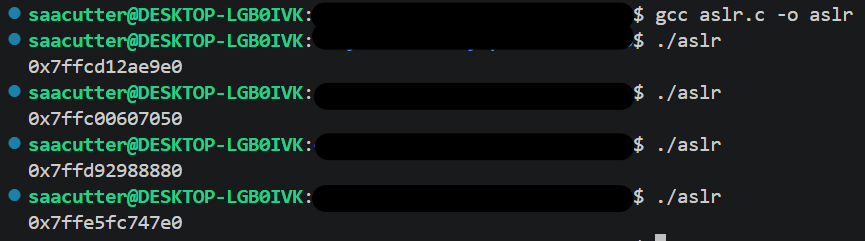
\includegraphics{aslr/aslr_demo.png}
\caption{aslr}
\end{figure}

ASLR is enabled by default on modern operating systems because
predictable memory addresses increase the reliability of memory-based
exploits. Disabling this feature typically requires altering the
operating system kernel and elevated privileges, so it is highly
recommended that this feature is never disabled.

\hypertarget{sandboxing}{%
\subsection{Sandboxing}\label{sandboxing}}

Sandboxing creates an isolated environment that can be used to safely
run/test/debug potentially malicious applications, proactively limiting
the damage that these applications can cause by restricting their
access. This is often done with some sort of virtualisation technique,
which attempts to isolate the sandbox environment from the host machine.
These environments are often temporary, but they can be configured to be
persistent depending on their purpose. There are a few different ways of
implementing sandboxes, including the use of virtual machines and
containerisation.

Virtual machines are emulations of physical computers, complete with
their own operating systems, applications, and allocated resources.
While this technique is primarily used to support multiple operating
systems on the same host, it also acts as a secure sandbox environment
that can be used to run potentially malicious applications. However,
these are incredibly resource intensive since they essentially act as a
second computer with its own allocation of CPU, RAM, storage, and
network bandwidth from the host.

For demonstration purposes, Windows Subsystem for Linux (WSL) 2 will be
utilised. This is a tool built into Windows 10/11 which allows Linux
distributions to be run directly on Windows in a lightweight virtual
machine. There are various distributions available on WSL, but for
testing purposes only Arch Linux and Ubuntu 24.04 will be used. After
these distributions are installed, they can be run using
\texttt{wsl\ -d\ {[}distribution{]}}. To confirm that different
operating systems are running, the \texttt{/etc/os-release} file can be
read.

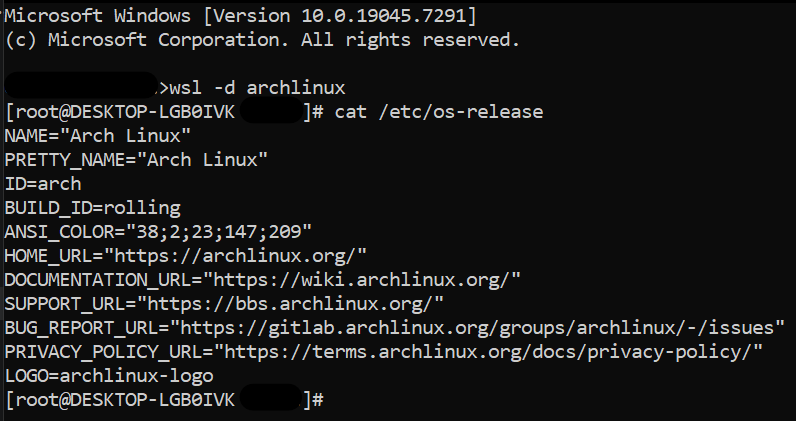
\includegraphics{sandboxing/sandbox_vm_arch.png}
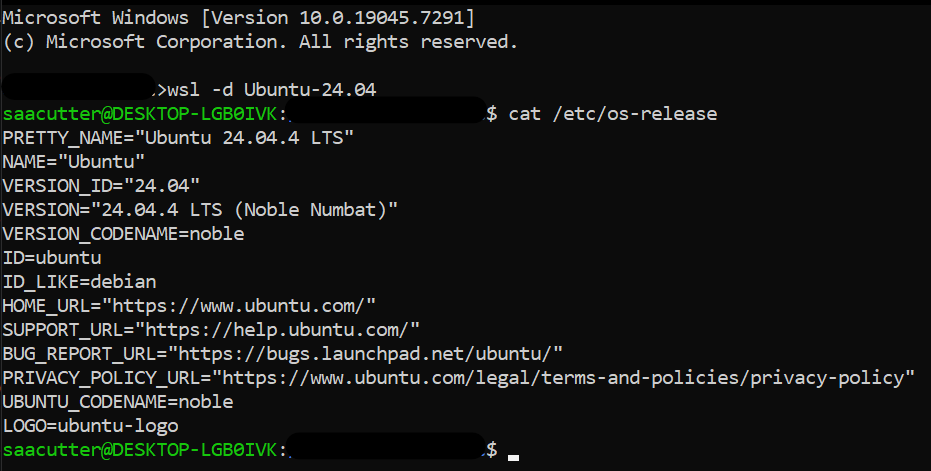
\includegraphics{sandboxing/sandbox_vm_ubuntu.png}

Containerisation puts applications into containers, which is essentially
a piece of software which packages up all the code and dependencies it
requires. Unlike virtual machines, these are lightweight and run as
isolated processes (meaning they can share the OS kernel with other
containers). These containers are also isolated from the host, meaning
that they can be used as a sandbox. The most common application which
supports containers is Docker, which is an open-source application.

There is a standard Ubuntu image available on Docker's servers, so this
can be used to demonstrate this isolation from the host. The Ubuntu
image can be pulled and run with
\texttt{docker\ run\ -it\ -\/-rm\ ubuntu}, which automatically opens up
an interactive shell. As both the container and host are running with an
Ubuntu shell, the easiest way to demonstrate this isolation is to list
the users. If the container exposes a different set of users from the
host system, this demonstrates that the container is operating in an
isolated environment.

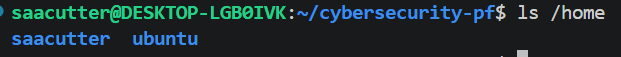
\includegraphics{sandboxing/sandbox_baseline.png}
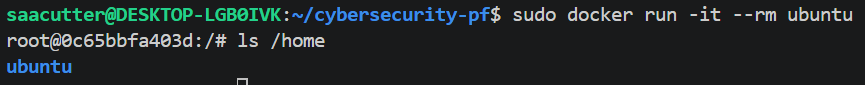
\includegraphics{sandboxing/sandbox_docker_ubuntu.png}

As shown, the Docker container only has one user (the \texttt{root}
Ubuntu user) while the host has two users (a personal user and the
\texttt{root} Ubuntu user) demonstrating separation from the host
environment.

\hypertarget{conclusion}{%
\section{Conclusion}\label{conclusion}}

Each of these mechanisms provides proactive defence against different
types of attacks. DEP prevents executable code from running in protected
memory regions, ASLR reduces the predictability of memory addresses used
by processes, and sandboxing isolates potentially malicious applications
from impacting the host environment. Although these protections can
sometimes be bypassed entirely through techniques like return-oriented
programming, they significantly increase the difficulty and complexity
of successful attacks.

\hypertarget{references}{%
\section{References}\label{references}}

Australian Signals Directorate. ``The case for memory safe roadmaps''.
Accessed: May 17, 2026. {[}Online{]}. Available:
https://www.cyber.gov.au/business-government/secure-design/secure-by-design/the-case-for-memory-safe-roadmaps

L. Danielson. ``What is ASLR? and why does it matter for
cybersecurity''. Huntress. Accessed: May 17, 2026. {[}Online{]}.
Available:
https://www.huntress.com/cybersecurity-101/topic/what-is-address-space-layout-randomization-aslr

N. Gupta. ``Demystifying ASLR: Understanding, Exploiting, and Defending
Against Memory Randomization''. Accessed: May 17, 2026. {[}Online{]}.
Available:
https://securitymaven.medium.com/demystifying-aslr-understanding-exploiting-and-defending-against-memory-randomization-4dd8fe648345

Hewlett Packard. ``Data Execution Prevention''. Accessed: May 19, 2026.
{[}Online{]}. Available:
https://h10032.www1.hp.com/ctg/Manual/c00387685.pdf

Advanced Micro Devices, Inc.~``AMD64 Architecture Programmer's Manual
Volume 3: General-Purpose and System Instructions''. Accessed: May 19,
2026. {[}Online{]}. Available:
https://docs.amd.com/v/u/en-US/24594\_3.37

Microsoft. ``Windows Sandbox''. Accessed: May 19, 2026. {[}Online{]}.
Available:
https://learn.microsoft.com/en-us/windows/security/application-security/application-isolation/windows-sandbox/

Microsoft. ``What is a Virtual Machine?''. Accessed: May 19, 2026.
{[}Online{]}. Available:
https://azure.microsoft.com/en-us/resources/cloud-computing-dictionary/what-is-a-virtual-machine

Microsoft. ``How to install Linux on Windows with WSL''. Accessed: May
19, 2026. {[}Online{]}. Available:
https://learn.microsoft.com/en-us/windows/wsl/install

Docker Inc.~``Use containers to Build, Share and Run your
applications''. Accessed: May 19, 2026. {[}Online{]}. Available:
https://www.docker.com/resources/what-container/
